\chapter{Etat de l'art}
\label{Chap2}
Les caractérisitiques des pièces produites grâce à la fusion laser sélective (SLM) sont le fruit de l'action simultanée et couplée d'un grand nombres de paramètres (voir figure \ref{fig:param} ) \parencite{Aboulkair140820}. Les résultats sont très sensibles à leurs variations et il est donc nécessaire de les contrôler méticuleusement. Pour ces raisons, il n'est pas simple d'étudier leurs impacts.\\

Durant les dernières années, les travaux visant à optimiser les conditions de fabrication se sont multipliés. La minimisation de la porosité est au centre de l'attention: elle est en effet liée à la qualité des propriétés mécaniques. De plus au delà d'un seuil, des risques de rupture prématurée peuvent apparaitre (source). (Initiation de sites de propag ... ) On s'intéresse ensuite à optimiser d'autres caractéristiques du matériau et à la productivité de la technique.


\begin{figure}[th]
\centering
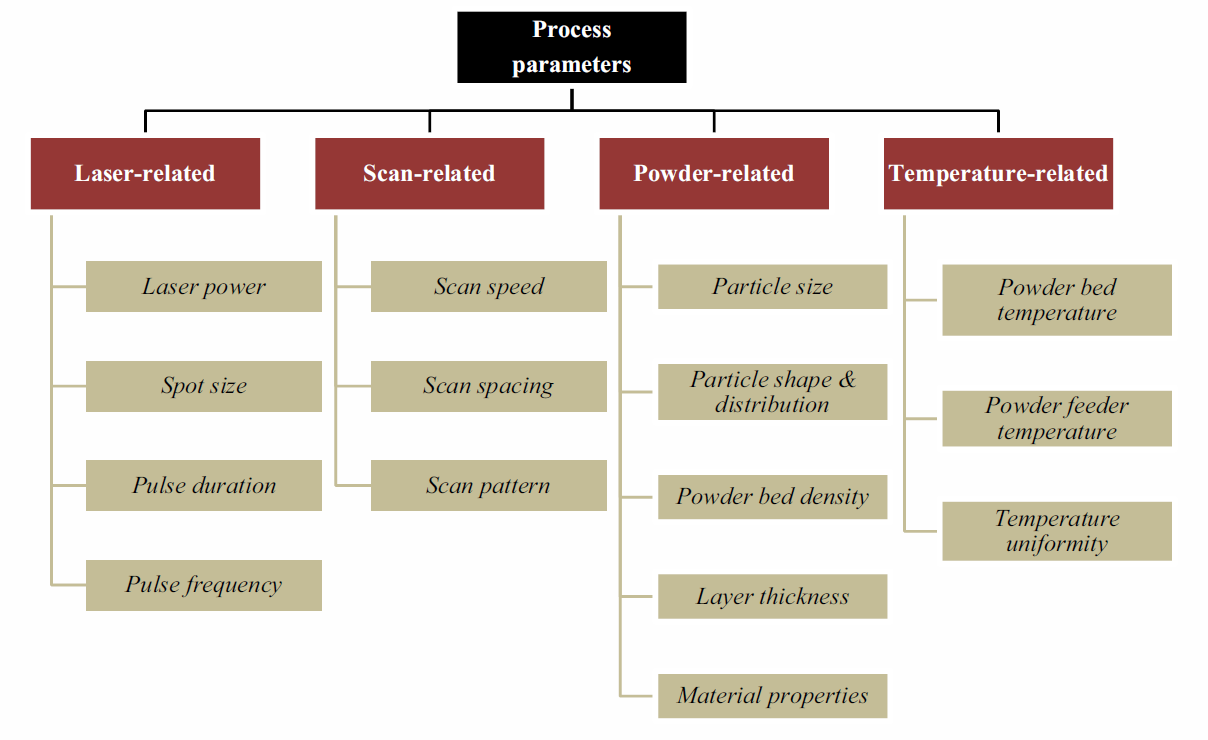
\includegraphics[scale=0.42]{Images/Param}
\decoRule

\caption[Paramètres entrant en jeu dans le procédé LSM]{Paramètres entrant en jeu dans le procédé LSM}
\label{fig:param}
\end{figure}

%Recherches biblio....
%\section{Comment référencer?}
%The \code{biblatex} package is used to format the bibliography and inserts references such as this one \parencite{Reference1}. The options used in the \file{main.tex} file mean that the in-text citations of references are formatted with the author(s) listed with the date of the publication. Multiple references are separated by semicolons (e.g. \parencite{Reference2, Reference1}) and references with more than three authors only show the first author with \emph{et al.} indicating there are more authors (e.g. \parencite{Reference3}). This is done automatically for you. %To see how you use references, have a look at the \file{Chapter1.tex} source file. Many reference managers allow you to simply drag the reference into the document as you type.
%
%Scientific references should come \emph{before} the punctuation mark if there is one (such as a comma or period). The same goes for footnotes\footnote{Such as this footnote, here down at the bottom of the page.}. You can change this but the most important thing is to keep the convention consistent throughout the thesis. Footnotes themselves should be full, descriptive sentences (beginning with a capital letter and ending with a full stop). The APA6 states: \enquote{Footnote numbers should be superscripted, [...], following any punctuation mark except a dash.} The Chicago manual of style states: \enquote{A note number should be placed at the end of a sentence or clause. The number follows any punctuation mark except the dash, which it precedes. It follows a closing parenthesis.}
%
%The bibliography is typeset with references listed in alphabetical order by the first author's last name. This is similar to the APA referencing style. To see how \LaTeX{} typesets the bibliography, have a look at the very end of this document (or just click on the reference number links in in-text citations).